\documentclass[output=paper]{langscibook}
\ChapterDOI{10.5281/zenodo.4727665}
\author{Piotr Pęzik\affiliation{University of Łódź}}
\title{Exploring the valency of collocational chains}
\abstract{Whereas the prefabricated status of idioms or restricted collocations is relatively self-evident in their context of use, the “underlying rigidity” \citep[110]{Sinclair1991} of other types of phraseological units may only become evident through large-scale analyses of reference corpora. This chapter focuses on the identification of subtle lexico-grammatical petrification of multiword units in dependency-annotated corpora. More specifically, it investigates restrictions on the valency of binary collocations and their tendency to be regularly subsumed by larger collocational chains. For example, the binary collocation \textit{deep breath} is almost invariably a direct object of a small set of verbs: \textit{take}, \textit{draw}, \textit{let out}. This restriction can be contrasted with collocational chains in which other adjectival collocations of \textit{breath} (e.g. \textit{bad breath}) have a wider range of syntactic roles determined mainly by the potential valency of their head noun (i.e. its propensity to function as subject, object etc.). Apart from discussing examples of such constructions from Polish and English corpus data, the chapter also attempts to show how lexico-syntactic properties of multiword units can be systematically accounted for and explored using a dependency-based approach to phraseology extraction.}

\begin{document}
\maketitle

\section{Introduction}

Since phraseology is a field ``bedevilled by the proliferation of terms and by the conflicting uses of the same term'' \citep[210]{Cowie1998}, it is not superfluous to clarify what is meant by the terms \textit{collocations} and \textit{collocational chains} in the context of this paper. Unless otherwise indicated, the term \textit{collocation} is taken to mean a \textit{binary lexical collocation}, i.e. a recurrent combination of just two content words (possibly linked by a grammatical word) which remain in an explicit syntactic relation, e.g. \textit{blind date}, \textit{turn of phrase}.  From the perspective of language production, collocations are assumed to be recalled from memory, either associatively or holistically, rather than recomposed in a completely spontaneous and uninspired manner. A review of different definitions of collocations by \citet{Pęzik2018} shows that they usually appeal to three main types of identification criteria: formal, distributional or psycholinguistic. The so-called ``restricted collocations'' are combinations which consist of an ``autosemantic'' base and a ``synsemantic'' collocate (\citealt{HeidGouws2006}). They can be roughly classified into four major groups \citep{Mel’čuk2001,Pęzik2018}. Open binary collocations are composed of two largely autosemantic words, which makes them less obvious to recognize as phraseological units. One of their subtle characteristics as units of prefabricated language is a degree of stereotyped recurrence, i.e. the tendency to occur in similar semantic, syntactic and pragmatic contexts \citep[51]{Pęzik2018}. While both restricted and open collocations play a key role in the production of fluent, native-like language, restricted collocations may also cause reception problems for non-native learners of a given language. Some restricted collocations are in fact figurative idioms as they instantiate conventionalized metaphors, metonymies and other conceptual blends, e.g. \textit{blind alley}.

There is a wide spectrum of phraseological units which may consist of more than two words, such as pure and figurative idioms, proverbs, commonplaces, catch phrases, slogans etc. \citep{Cowie1998}. Although tens of thousands of idioms and collocations have been identified and recorded in dictionaries and combinatorial databases, there is a need for further research on some of the more subtle types of phraseological prefabrication. Among the less extensively researched phraseological phenomena are collocational chains, which are defined here as overlapping combinations of two or more lexical collocations.\footnote{Some definitions of collocational chains also distinguish between collocational chains and collocational clusters \citep{Hausmann2004,HeidGouws2006}.} As shown further in this paper, collocational chains can be composed ad hoc or they are largely predetermined to occur in their entirety.

Defining collocations and other types of phraseological units (PUs) as word combinations linked by an explicit syntactic relation may come across as somewhat controversial, partly because the syntactic idiosyncrasy of PUs is regularly mentioned as one of their most salient characteristics. In its extreme form it can be described as \textit{ill-formedness} or deviation from grammatical regularity. For example, the fact that it is difficult to assign the constituents of the idiomatic expression \textit{by and large} to modern day English morphosyntactic categories has earned it the name of ``an ill-formed collocation'' \citep{Moon1998}.\footnote{Such highly idiosyncratic combinations are difficult to directly integrate in the standard dependency representation used for the proposed method of phraseology extraction.}  More often, phraseological units tend to be petrified in that they are mostly used in a limited subset of the morphological variants licensed by their otherwise regular syntactic structure. However, although syntactic idiosyncrasy testifies to the status of some PUs as clearly prefabricated constructions, one should not conclude that all or even most PUs are marked by syntactic irregularity. In reality, most idioms and collocations seem to be lexical realizations of regular syntactic patterns, even if their prototypical forms are petrified. The most obvious proof of this statement is the existence of dictionaries of idioms (\citealt{CowieMackin1975,CowieEtAl1993}) and collocations \citep{CrowtherEtAl2003} whose macro- and microstructures are organized around a set of productive syntactic patterns of idiomatic expressions. Furthermore, the very fact that most subsentential PUs have to be embedded in the syntactic structure of a sentence means that they also have an ``external valency'' \citep{Burger2003}. To put it in the parlance of dependency syntax, PUs have typical syntactic roles as governors or dependents of other words and phrases in the sentence. Those two properties of PUs, i.e. their internal structure and external valency are implicitly recognized in combinatorial dictionaries as illustrated in the following entry for the phrasal verb \textit{to back on to} from the Oxford Dictionary of Current Idiomatic English (\citealt{CowieMackin1975}: 10):

\ea
back on to [A3] \textit{have at its back, face at the back}. \textbf{S}: house, shop; study, kitchen. \textbf{o}: court-yard; lane, alley
\z

The internal structure of the phrasal expression is indicated by the label A3, which denotes intransitive verbs with a particle and a preposition, while its external valency is implied by the two lists of its typical subjects (S) and objects (o).

The assumption that most phraseological units have both a regular internal syntactic structure and an external valency specification opens up some possibilities for computerized explorations of their distribution as either self-contained or largely embeddable constructions. This point is elucidated at some length in the subsequent sections of this paper, but it can be illustrated right away with a simple example. In reference corpora of English, the seemingly independent binary collocation \textit{profound effect} functions almost exclusively as a direct object of \textit{have} as in \textit{have a profound effect}. The latter construction is in turn subsumed by an even longer collocational chain with \textit{on} as a fixed prepositional dependent and its open-ended prepositional nominal or pronominal object dependent as in \textit{to have a profound effect on} + NOUN/PRON. The fact that such structures may be recursively recombined in multiple, possibly also prefabricated constructions has some practical implications for the design of phraseological dictionaries and databases. 

This paper first discusses the problem of fragmentation of such collocational chains in dictionaries and automatic combinatorial databases. The phenomenon of syntactically restricting subsumption of shorter word combinations in longer recurrent constructions is then discussed  in terms of potential valency restrictions. Finally, the paper presents a new software tool named Treelets\footnote{See \url{http://pelcra.pl/new/treelets}.}, which showcases some applications of dependency-based phraseology extraction. The method of generating a combinatorial dictionary implemented in this tool uses special data structures called \textit{subsumption graphs} to facilitate the search and visualization of embedded and overlapping phraseological constructions.

\section{Relational phraseology extraction}
\subsection{Fragmentation of phraseological units}

The degree to which various PUs can be expected to adhere to regular syntactic structure is important in the context of phraseology extraction (PE) -- an area of corpus research which deals with automated identification of phraseological units in corpora through aggregation of word co-occurrences attested in reference corpora. PE techniques can be broadly categorized into positional and relational \citep{Evert2005}, although this distinction is sometimes blurred by practical considerations. Positional approaches rely on counting and weighing linearly related word co-occurrences in text. Relational PE techniques utilize explicit annotations of syntactic relations between constituents of PUs. As a result, the latter type of methods crucially depend on the syntactic predictability of PUs; word combinations which co-occur in syntactic configurations unpredicted by predefined syntactic patterns are ignored in the process of extraction. Because syntactic patterns used in the process of extraction have to a) conform to the particular treebank formalism used to annotate the working corpus and b) be consistently annotated by automatic syntactic parsers, the results of relational extraction may reveal only “details of language” covered by a particular syntactic theory \citep[4]{Sinclair1991} rather than the full spectrum of usage.

\begin{table}[b]
\begin{tabular}{cl S[table-format=3.1] S[table-format=2.2] S[table-format=2.5] S[table-format=3.3] S[table-format=1.2]}
\lsptoprule
{\#} & {Collocate} & {Frequency} & {T-score} & {MI\textsuperscript{3}} & {G\textsuperscript{2}} & {JD}\\
\midrule
1 & competitive & 149 & 11.57 & 18.71 & 613.96 & 0.82\\
2 & full & 166 & 8.43 & 16.28 & 139.45 & 0.90\\
3 & added & 71 & 8.12 & 17.09 & 346.23 & 0.84\\
4 & comparative & 68 & 7.89 & 16.72 & 308.08 & 0.72\\
5 & unfair & 67 & 7.69 & 16.21 & 260.58 & 0.85\\
\lspbottomrule
\end{tabular}
\caption{\label{tab:pezik:2} Adjectival collocates of \textit{advantage} recorded in HASK EN database}
\end{table}

Another broad distinction can be made between ``ad hoc'' PE modules and extraction systems which precompute combinatorial databases with a dictionary-like macrostructure. Ad hoc PE modules available in various corpus search engines usually perform positional extraction of binary collocations, n-grams or skip-grams for single and multiterm queries defined by users. For example, the collocation extraction of the MoncoEN corpus search engine\footnote{See \url{http://monco.frazeo.com.}} can be used to define a single- or multiword node expression for any corpus query formulated in its query syntax. \tabref{tab:pezik:1} (overleaf) presents a list of adjectival collocates extracted from a sample of almost 70,000 occurrences of the noun \textit{advantage} in data crawled from various English-language news websites. The results of the extraction query can be sorted by frequency or their strength of association, which is a variation of the Dice score in this case. The fourth column contains a frequency list of positions relative to the node word (which occurs at position=0) which is useful in identifying the predominant syntactic roles of the collocates. For example, the adjective \textit{competitive} seems to mainly precede the noun \textit{advantage}, which suggests that it is used as an adjectival premodifier in this case. The last column lists word n-grams bounded by the node and collocate, which is meant to indicate some of the recurrent forms of each collocation as well as its higher-order constructions such as noun phrases with multiple adjectival modifiers, e.g. \textit{unfair competitive advantage}.

\begin{sidewaystable}\small
\begin{tabularx}{\textwidth}{llrrlQ}
\lsptoprule
\# & Adjective & Frequency & Dice & Positions & Example n-grams\\\midrule
1 & competitive &  1260 &  0.0413 & \{-1=1239, -2=17, 2=4\} & \{competitive advantage=1078\},\{competitive advantages=161\},\{competitive business advantage=3\}\\
\tablevspace
2 & full &  1165 &  0.0382 & \{-1=1154, -2=9, 2=2\} & \{full advantage=1134\},\{fullest advantage=12\}, \{full advantages=4\},\{fuller advantage=3\},\{full of advantage=3\\
\tablevspace
3 & big &  900 &  0.0295 & \{-2=76, -1=789, 2=34, 1=1\} & \{big advantage=488\},\{biggest advantage=167\},\{big advantages=75\},\{advantage of big=14\},\{big an advantage=5\},\{big size advantage=5\},\{big fundraising advantage=4\},\{biggest home-field advantage=3\}\\
\tablevspace
4 & unfair &  643 &  0.0211 & \{-1=567, 2=2, -2=74\} & \{unfair advantage=525\},\{unfair advantages=42\},\{unfair competitive advantage=34\},\{unfair commercial advantage=5\},\{unfair trade advantage=4\},\{unfair competitive advantages=4\}\\
\tablevspace
5 & great &  571 &  0.0187 & \{-1=456, 2=41, -2=74\} & \{great advantage=320\},\{great advantages=92\},\{greater advantage=37\},\{advantage of great=23\},\{great comparative advantage=9\},\{advantage , great=7\},\{greater advantages=7\},\{great natural advantages=6\},\{great competitive advantage=5\}\\
\lspbottomrule
\end{tabularx}
\caption{\label{tab:pezik:1} Adjectival collocates of \textit{advantage} retrieved with the MoncoEN search engine}
\end{sidewaystable}


\hspace*{-.5mm}\tabref{tab:pezik:2} shows the top five adjectival collocates of the noun \textit{advantage} recor\-ded in HASK EN (Pęzik 2014),\footnote{See also \url{http://pelcra.pl/hask\_en}.} a combinatorial database precomputed from the original edition of the British National Corpus (BNC). The remaining columns of the table show a selection of strength of association and dispersion scores.



Even though all of the top adjectives from the two lists seem to be genuine collocates of the noun \textit{advantage}, both of the extraction systems illustrated above suffer from the problem of fragmentation: recurrent fragments of larger multiword expressions are represented as unrelated binary collocations. For example, taken at face value, both of the lists above might imply that \textit{full advantage} is a self-contained intensifying binary collocation which could be used freely in a variety of syntactic roles predetermined by its head noun. However, in the first edition of the British National Corpus (BNC) more than 86\% of the occurrences of \textit{full advantage} function as part of the longer expression \textit{take full advantage} (\textit{of}). In a 440 million word version of the Corpus of Contemporary American English (COCA) the same phrase is used as a direct object of \textit{take} in over 96\% of its attested usages. In other words, \textit{full} seems to function as a collocational intensifier of \textit{advantage} mostly when the latter is a direct object of the light verb construction \textit{take} + \textit{advantage} as illustrated in \REF{ex:pezik:2} :

\ea
\textit{Customers \textbf{\textit{take} \textbf{full} \textbf{advantage}} of in-house electropolishing (...).} [COCA, \textit{Physics Today}]\label{ex:pezik:2}
\z

Intended users of such tools and automatically extracted resources are therefore required to inspect the concordances underlying such tabular results to distinguish between mostly subsumed collocations and freely recombinable collocations such as \textit{big advantage}. The latter combination is not restricted to occurring in a single syntactic function. It is used as a direct object of verbs such as \textit{have} or \textit{give} in approx. 34\% of its occurrences in COCA and as a nominal subject dependent (28\% of occurrences) as in \REF{ex:pezik:3}:

\ea
\textit{The \textbf{\textit{big} \textbf{advantage}} for the investor \textbf{\textit{is}} that he can trade all his cryptocurrencies in one place.} [MoncoEN, thenextweb.com]\label{ex:pezik:3}
\z

Collocation dictionaries may also be affected by the problem of PU fragmentation. For example, the \textit{Oxford Dictionary of Collocations} \citep{CrowtherEtAl2003}, henceforth the ODC, defines the noun \textit{bearing} as a ``way in which something is related'' and lists three of its adjectival collocates: \textit{direct}, \textit{important} and \textit{significant}. None of those collocations is likely to be used outside of the larger construction \textit{have a} \textit{direct\slash important\slash significant} \textit{bearing on}. This information is only indirectly implied by the example sentence illustrating the use of the first of those collocations and a separate entry for the direct object lexical collocation of \textit{have} + \textit{bearing} and the grammatical collocation of \textit{bearing} + \textit{on}:

\ea
bearing

1. \textit{way in which sth is related}

ADJ. \textbf{direct,} \textbf{important,} \textbf{significant} 

\textit{The rise in interest rates had a direct bearing on the company's profits.}

VERB\,+\,BEARING  \textbf{have}

PREP. {\textasciitilde} \textbf{on}
\z

Of course, the coverage of this particular dictionary was by design limited to binary collocations and its space limitations preclude detailed usage notes. On the other hand, it could be argued that this collocational chain would probably be better represented as a single unit in this case. In the OCD a special section labelled \textit{PHRASES} is occasionally used to enumerate additional fixed expressions which do not conform to the four basic patterns of binary collocations covered by this dictionary.

\tabref{tab:pezik:3} shows more examples of intensifying adjectival modifier collocations which are rarely, i.e. usually in less than 15\% of cases, used independently of larger, recurrent constructions. 

\begin{sidewaystable}\small
\begin{tabularx}{\textwidth}{l@{ }lrrccQ}
\lsptoprule
{\#} & {Binary AMOD coll.} & \multicolumn{2}{c}{Frequency} & \multicolumn{2}{c}{Subsumption as DOBJ} & Frequent verb governors in (COCA; BNC)\\\cmidrule(lr){3-4}\cmidrule(lr){5-6}
&  & {BNC} & {COCA} & {BNC} & {COCA}\\\midrule
1 & upper hand         & 122 & 670  & 122/122=1 & 608/670=0.91 & have (36; 223), gain (41; 157), get(19; 100), give (8; 36), hold(8; 25) + the upper hand\\
\tablevspace
2 & little resemblance & 59  & 208  & 57/59=0.966 & 181/208=0.93 & bear (56; 181) + little resemblance\\
\tablevspace
3 & mental note        & 78  & 289  & 75/78=0.96  & 262/289=0.90 & make (74; 228), take (1; 20) + a mental note\\
\tablevspace
4 & deep breath        & 664 & 4,282 & 587/664=0.88 & 3872/4282=0.89 & take (505; 3438), draw (72; 225), let out (7; 30) + a deep breath\\
\tablevspace
5 & important bearing  & 30  & 14   & 30/30=1 & 14/14=1 & have (30; 14) + an important bearing\\
\tablevspace
6 & profound effect    & 164 & 460  & 156/164=0.95 & 420/460=0.91 & have (150; 392) + profound effect\\
\tablevspace
7 & significant role   & 146 & 905  & 129/146=0.88 & 824/905=0.91 & play (105; 692), have (15; 66) + a significant role\\
\tablevspace
8 & full advantage     & 170 & 423  & 146/170=0.86 & 406/423=0.96 & take (142; 402) + full advantage\\
\tablevspace
9 & excellent job      & 58  & 326  & 49/58=0.85 & 306/326=0.94 & do (46; 298) + an excellent job\\
\tablevspace
10 & short laugh       & 72  & 100  & 72/82=0.88 & 74/100=0.74 & give (67; 43) + a short laugh\\
\lspbottomrule
\end{tabularx}
\caption{\label{tab:pezik:3}Examples of binary adjectival modifier collocations regularly embedded in larger collocational chains in BNC and COCA}
\end{sidewaystable}

The first example ``collocation'' in the second column of \tabref{tab:pezik:3} is \textit{upper hand}. In the BNC it is always used as a direct object of a handful of verbs shown in the last column (\textit{have}, \textit{gain}, \textit{give}, \textit{hold}) while in COCA there are sporadic instances of usage as implicit direct objects in elliptic headlines or in other syntactic roles. A similar level of subsumption is observed for the phrase \textit{mental note} which is rarely used outside of the set expressions \textit{make\slash take a mental note}. Non-direct object usage requires a creative context such as science-fiction writing, as illustrated in \REF{ex:pezik:5}:

\ea
\textit{Amber put it on her mental note pad. [COCA, Analog Science Fiction \& Fact]} \label{ex:pezik:5}
\z

Some of the examples from \tabref{tab:pezik:3}, such as \textit{have the upper hand} and \textit{take a mental note} are simply multiword figurative idioms and thus the problem of their identification as phraseological units is purely technical. On the other hand, example phrases 5 (\textit{direct bearing}, which is invariably embedded in \textit{have a direct bearing} in the two corpora), 6 (\textit{profound effect}), and 7 (\textit{significant role}) are restricted intensifying collocations. Examples 9 (\textit{excellent job}) and 10 (\textit{short laugh}) are open collocations comprised of two largely autosemantic constituents which simply happen to regularly form a longer structure with an overlapping direct object collocation. The typological dilemma with the latter examples is therefore whether they should be recognized as self-contained phraseological units or as more spurious and open-ended constructions. For the practical purposes of phraseology extraction, we might describe the frequently embedded phrases as \textit{subsumed binary collocations}, depending on how unlikely they are to be used independently of the larger constructions. The subsuming constructions can be multiword idioms or simply recurrent collocational chains. Collocational chains which consist of subsumed collocations should be distinguished from spurious chains of independent collocations such as \textit{my heart of stone is filled with pride}.\footnote{See \url{https://www.youtube.com/watch?v=wvYRQ-sFMJw} (2:18).}

As shown in \tabref{tab:pezik:4} some of the amod\,+\,dobj (an adjectival modifier followed by a direct object) constructions from \tabref{tab:pezik:3} are highly likely to occur in larger recurrent structures which are also subtrees of the sentence dependency tree. For instance, more than 87\% of the occurrences of the recurrent chain \textit{play a significant role} in COCA have a prepositional object (pobj) introduced by \textit{in} as in \textit{play a significant role in} + pobj. The subsumption of the other four second-order chains shown in \tabref{tab:pezik:4} in third-order chains is even higher in the two reference corpora.

\begin{table}
\begin{tabularx}{\textwidth}{l@{ }Qrrcc@{ }l}
\lsptoprule
   &  & \multicolumn{2}{c}{{Frequency}} & \multicolumn{3}{c}{Used with a pobj dependent}\\\cmidrule(lr){3-4}\cmidrule(lr){5-7}
\# & {amod} {+} {dobj} {collocational} {chain} & {BNC} & {COCA} & {BNC} & {COCA}\\
\midrule
1 & play a significant role & 105 & 692 & 92/105=0.88 & 616/692=0.89 & (in)\\
2 & bear little resemblance & 59 & 181 & 52/59=0.88 & 175/181=0.97   & (to)\\
3 & have a direct bearing & 37 & 54 & 33/37=0.89 & 54/54=1           & (on/upon)\\
4 & have profound effect & 150 & 392 & 133/150=0.89 & 348/392=0.89   & (on/upon)\\
5 & take full advantage & 142 & 402 & 132/142=0.93 & 380/402=0.95    & (of)\\
\lspbottomrule
\end{tabularx}
\caption{\label{tab:pezik:4} Subsumption of \textit{amod\,+\,dobj} collocational chains in structures with a prepositional attachment}
\end{table}

\subsection{Potential vs. activated valency of PUs}

The subsumption of shorter dependency subtrees (including single word subtrees) in longer recurrent collocational or idiomatic structures may considerably affect the distribution of their syntactic roles. As an example, the noun \textit{fact} appears as a prepositional object much more frequently than the ratio of all nouns used as prepositional objects in reference corpora of English. However, the ratio of \textit{fact} as a prepositional object drops approximately to the level observed for all nouns when \textit{fact} is modified by an adjective (see the discussion of Tables~\ref{tab:pezik:5}--\ref{tab:pezik:7} below). More generally, dependency type ratios vary considerably not only for different content words but also with respect to the higher order constructions in which they occur.

\hspace*{-.2mm}In dependency syntax, vertices representing words in the sentence dependency tree can be said to have a ``passive valency'' (\citealt{Melʹčuk1988}, cf. \citealt{Boguslavsky2003,Boguslavsky2016,Boguslavsky2003}). The passive valency of a dependency subtree (including single-word subtrees with their morphosyntactic roles such as nouns, verbs, adjectives etc.) can be defined as its default propensity to function as a governor or dependent of a set of types. Since the terms ``active'' and ``passive valency'' have also been used to refer to the direction of the dominance relationship between words in a dependency tree \citep{Moroz2013}, to avoid confusion in this paper, the terms \textit{potential} and \textit{activated valency} will be used to describe the default and corpus-attested dependency patterns formed by words and phrases. For example, nouns have the rather obvious default potential of functioning as nominal subjects, objects of verbs or prepositions, nominal modifiers etc., while verbs are typically sentence roots, auxiliaries, x-complements etc. The approximate activation of such potential valency roles  (i.e. the activated valency of a word or phrase) can be estimated from manually annotated dependency treebanks or automatically parsed corpora. Neither of these options is ideal as treebanks are limited in size and parsers produce erroneous annotations, but even an approximate estimation of the activated valency of a word or phrase may throw some light on its actual usage.

As shown in \tabref{tab:pezik:5}, in both COCA and BNC, nominal dependents are usually prepositional objects (35--38\% of all noun occurrences), direct objects (16\%) and nominal subjects (12--18\%).

\begin{table}
\begin{tabular}{l rrr  rrrr}
\lsptoprule
& \multicolumn{2}{c}{BNC} & \multicolumn{4}{c}{COCA}\\\cmidrule(lr){2-3}\cmidrule(lr){4-7}
Dep. type & Freq. & Ratio & Freq. & Ratio & M/n\footnote{Mean per noun} & SD\\\midrule
pobj      &  7 844 932 &  0.38 & 30 824 682 &  0.35 &  0.20 &  0.34\\
dobj      &  3 246 866 &  0.16 & 14 922 242 &  0.16 &  0.09 &  0.24\\
nsubj     &  2 416 031 &  0.18 & 10 870 549 &  0.12 &  0.10 &  0.25\\
compound  &  2 008 918 &  0.09 & 9 787 999  &  0.11 &  0.15 &  0.31\\
conj      &  1 550 954 &  0.07 & 5 509 718  &  0.06 &  0.08 &  0.22\\
attr      &  853 480   &  0.04 & 3 728 782  &  0.04 &  0.02 &  0.13\\
nsubjpass &  579 565   &  0.03 & 1 474 911  &  0.01 &  0.06 &  0.21\\ 
ROOT      &  533 112   &  0.02 & 3 068 416  &  0.03 &  0.01 &  0.07\\
npadvmod  &  474 680   &  0.02 & 2 537 174  &  0.02 &  0.12 &  0.30\\
appos     &  305 757   &  0.01 & 2 215 588  &  0.02 &  0.02 &  0.12\\ 
\lspbottomrule
\end{tabular}
\caption{\label{tab:pezik:5}Ten most frequent types of nominal dependents in BNC and COCA}
\end{table}

The most common dependents of English nouns are determiners (24.6\%), followed by adjectival modifiers (16.6\%) and prepositions (12.2\%). The proportions of dependency relation types for specific nouns, verbs or adjectives may differ significantly from such overall distributions. As shown in the last column of \tabref{tab:pezik:5}, the standard deviation of the prepositional object dependent type is 0.34 percentage points in COCA. 

In studies of verb valency, it is taken for granted that different verbs can be classified into groups of similar subcategorization frames. In other words, different verbs require or subcategorize different types of configurations of their dependents. From the perspective of phraseology, it is also interesting to consider the activated valency of nouns and other open-class content words such as adjectives or adverbs which function as headwords defining the entry structure of lexicographic resources. The activated valency of a dependency subtree (such as a word or phrase) can be defined as the set of dependent and governor types in which it is found in a reference corpus. Although corpus-based valency estimations can only be probabilistic and approximate in nature, they do shed light on the actual usage patterns of words and phrases, and they are especially revealing when such words or phrases tend to be embedded in larger recurrent constructions.

\tabref{tab:pezik:6} shows the distribution of dependent types realized by the nouns \textit{breath} and \textit{fact} estimated from the syntactically annotated version of COCA used in this study. The use of \textit{breath} as a direct object is considerably more frequent than the average value observed for nouns in this corpus (49.95 vs. 16.8\%), whereas its frequency as a prepositional object is lower than the average (29.54 vs. 34.12\%). On the other hand, the noun \textit{fact} is a prepositional object in over 65\% of its occurrences, which is considerably higher than the average ratio of 34\% observed for all nouns in this corpus. This example shows that the activated valency of those two words tends to differ considerably either from their potential valency as nouns or even from the overall or average rations observed for all nouns in a reference corpus.


\begin{table}[t]
\begin{tabular}{lrr lrr}
\lsptoprule
\multicolumn{3}{c}{\textit{breath} {in} {COCA}} & \multicolumn{3}{c}{\textit{fact} {in} {COCA}}\\
\cmidrule(lr){1-3}\cmidrule(lr){4-6}
Dep. type & {Freq.} & {Ratio} & {Dep.} {type} & {Freq.} & {Ratio}\\\midrule
dobj &  12,830 &  0.50 & pobj &  108,026 &  0.67\\
pobj &  7,589 &  0.30 & nsubj &  18,964 &  0.12\\
nsubj &  2,344 &  0.09 & dobj &  16,150 &  0.10\\
compound &  851 &  0.03 & attr &  7,336 &  0.04\\
conj &  520 &  0.02 & conj &  3 657 &  0.02\\
\lspbottomrule
\end{tabular}
\caption{\label{tab:pezik:6} The nouns \textit{breath} and \textit{fact} as dependents in COCA}
\end{table}

It is not obvious whether the difference between the typical dependency types of the two nouns can be linked to their general semantic properties. What seems to be the case is that at least \textbf{some} of this variation is due to a handful of phraseological restrictions on the valency of those two nouns. For example, almost 72\% of all the occurrences of \textit{breath} as a direct object are governed by just four verbs: \textit{take} (5,194), \textit{hold} (1,896), \textit{catch} (1,428), \textit{draw} (708). Taken alone, the support verb restricted collocation \textit{take a breath} accounts for over 40\% of the use of \textit{breath} as a direct object. The syntactic distribution of the noun \textit{fact} is even more biased by its formulaic usage: over 64\% (69,295) of its occurrences as a prepositional object  \textit{fact} are instances of a single discourse linking phrase: \textit{in fact}. 

The activated valency levels observed for a single word may change considerably once this word in used in a collocation. The previous section shows how the potential valency of binary collocations may also be restricted by the distribution of a small set of prefabricated higher order structures in which they are typically found. \tabref{tab:pezik:7} shows frequencies of dependent types assumed by the nouns \textit{fact} and \textit{breath} when they are modified by adjectives as in [\textit{access}] \textit{simple facts} or \textit{have bad breath}. The proportion of individual dependency types of the two nouns is only partly consistent with their overall dependency type distribution. Adjective-modified occurrences of \textit{breath} are even more likely to be direct objects (68\%), whereas instances of \textit{fact} with an adjectival modifier are half as likely to be prepositional objects. Much of the first difference can be explained by the existence of the construction \textit{take a deep breath}, which is used both literally as an established collocational chain and idiomatically as a figurative expression (see \tabref{tab:pezik:3}).  The decrease in the ratio of prepositional object instances of \textit{fact} observed when we consider its use with adjectival modifiers results to a large extent from the absence of \textit{in fact} or a similar phrase in this ranking. There are some formulaic adjective-modified usages of \textit{fact} as a prepositional object such as the sentence initial discourse marker \textit{in actual fact} (67 occurrences in COCA), but they do not compensate for the absence of the much more frequent prepositional phrase \textit{in fact}. The propensity of a word or phrase to be used as a dependent or governor of a larger structure may be significantly skewed by its use in a single higher-order phraseological construction such as \textit{take a deep breath} or \textit{in fact}. 

\begin{table}
\begin{tabular}{lrr lrr}
\lsptoprule
\multicolumn{3}{c}{amod(fact, x)} & \multicolumn{3}{c}{amod(breath, x)}\\\cmidrule(lr){1-3}\cmidrule(lr){4-6}
 {Type} & {Freq.} & {Ratio} & {Type} & {Freq.} & {Ratio}\\\midrule
Pobj &  3,333 &  0.32 & dobj &  6,033 &  0.68\\
Dobj &  2,247 &  0.21 & pobj &  1,824 &  0.21\\
Nsubj &  1,870 &  0.18 & nsubj &  314 &  0.04\\
Attr &  1,332 &  0.13 & ROOT &  171 &  0.02\\
Conj &  401 &  0.04 & conj &  163 &  0.02\\
\lspbottomrule
\end{tabular}
\caption{\label{tab:pezik:7}Top five dependent types \textit{fact} and \textit{breath} with a modifying adjective}
\end{table}

In order for automatic combinatorial databases to account for activated valency patterns of phraseological units, they have to identify and represent such subsumption phenomena. The following section describes a method of storing extracted collocational structures which was designed to address the issue of recursive subsumption of PUs. 

\subsection{Subsumption graphs}

\citet{Pęzik2018} describes an experimental method of extracting combinatorial data\-bases from dependency-parsed corpora which keeps track of subsumption relations between overlapping constructions of different sizes. The working assumption of the PE approach used in this study is known as the continuity restraint \citep{OGrady1998}, which predicts that an idiom’s obligatory lexical components form a subtree of the sentence dependency tree. The validity of this assumption depends on the exact dependency formalism used to represent PUs. Also, it seems to fail in the case of some variable idiomatic expressions such as \textit{walk a thin{\textbar}fine line{\textbar}path between}. It is nevertheless a useful assumption in large-scale phraseology extraction. One of its advantages is that it covers collocational subtrees which are neither complete or single phrasal constituents such as \textit{include such factors as}.

The extraction process starts with a set of headwords, which are simply part-of-speech typed lemmas of content words, and a set of dependency patterns in which those headwords are expected to occur. Next, for each headword, the full set of lexically recurrent subtrees, ``catenae'' \citep{OsborneEtAl2012} or ``treelets'' is extracted from a reference corpus. Extracted subtrees are stored with some distributional and structural properties in a relational database. The headwords define the macrostructure of the resulting automatic combinatorial dictionary (ACD) and the set of patterns used determines the microstructure of each of its entries.

\begin{figure}[b]
% 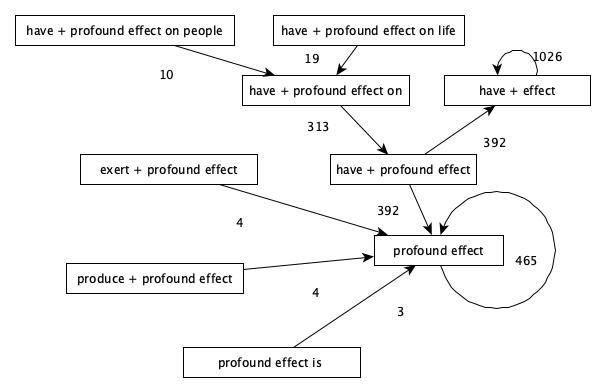
\includegraphics[width=\textwidth]{figures/pezik-img001.png}
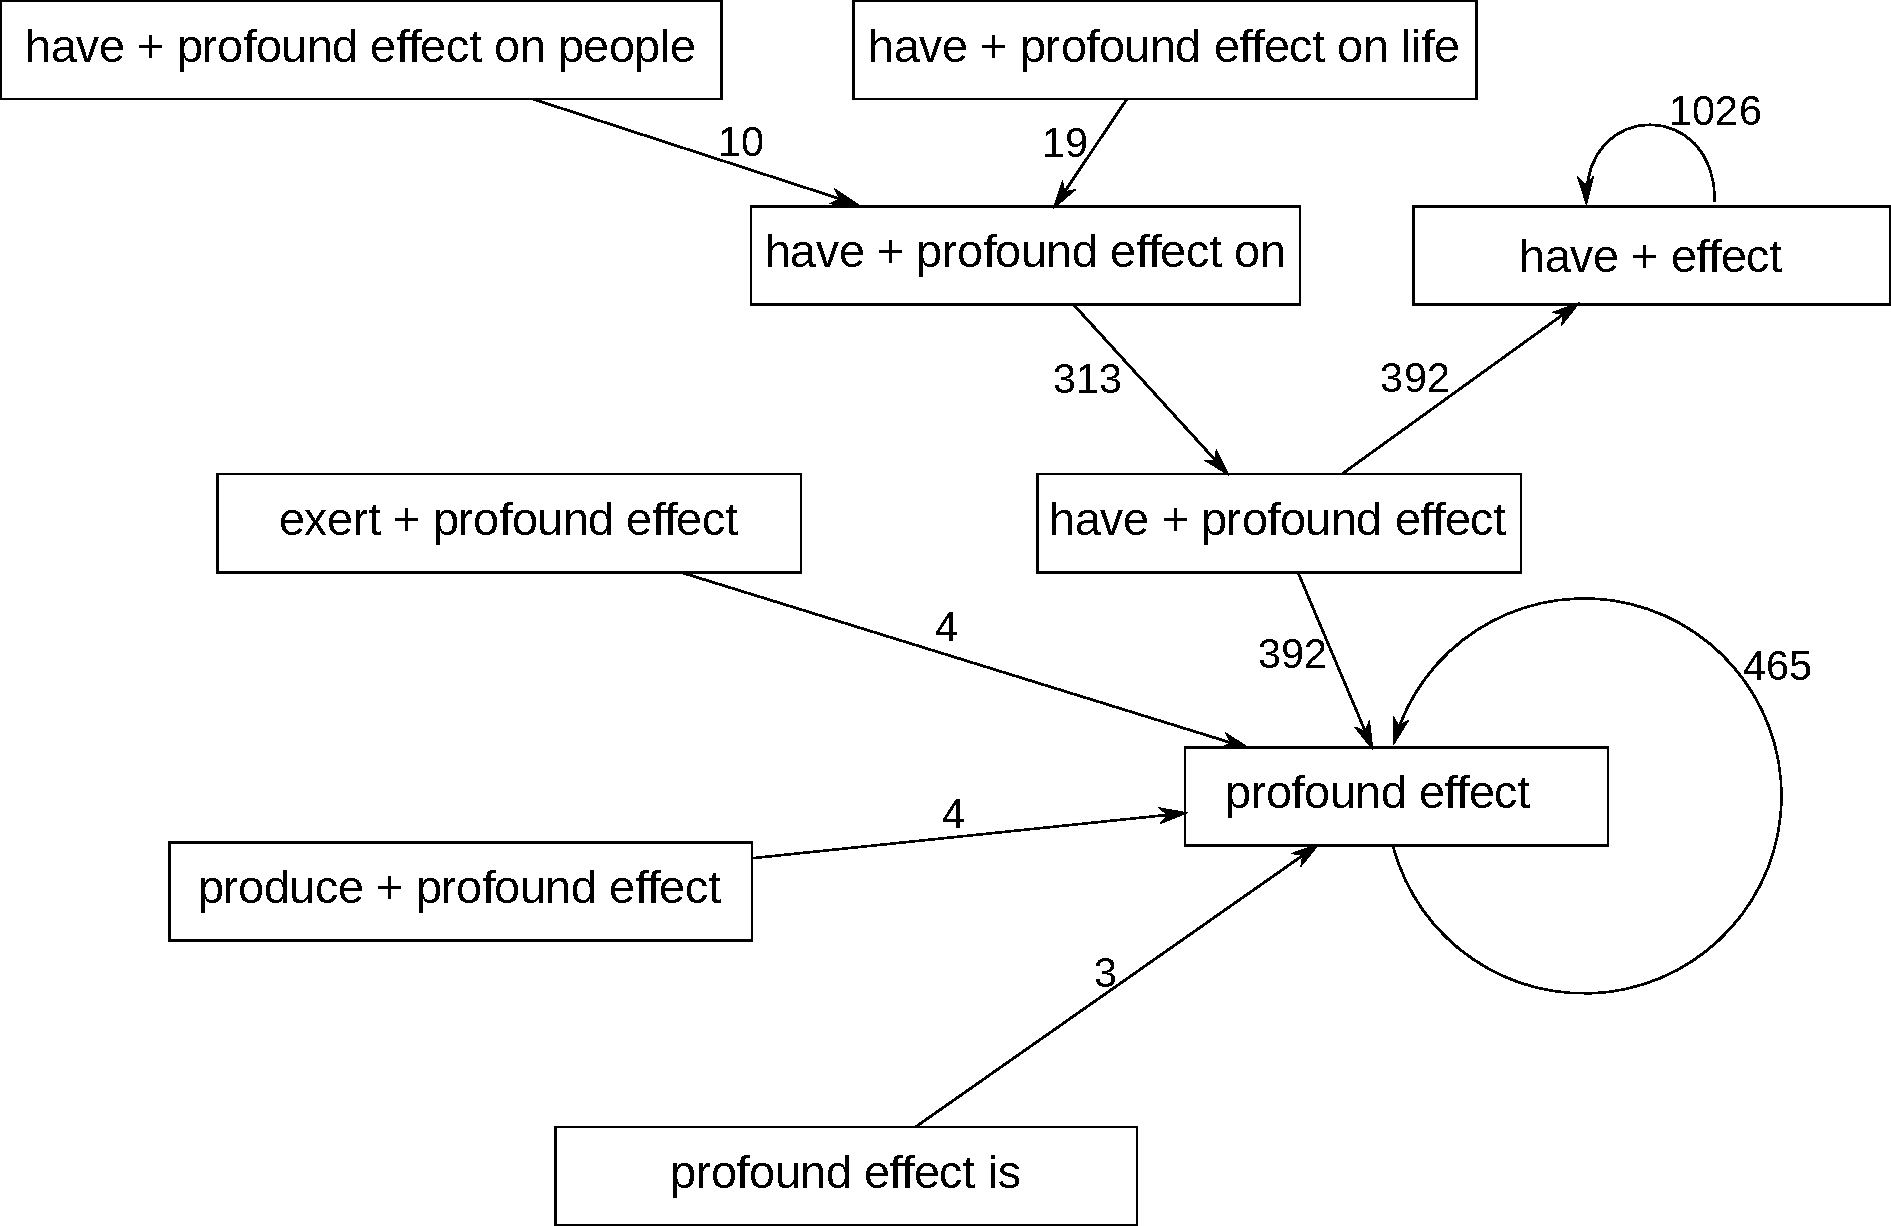
\includegraphics[width=\textwidth]{figures/pezik1.pdf}
\caption{A simplified subsumption graph generated for recurrent dependency subtrees containing the noun \textit{effect} in COCA. Only a subset of recurrent subtrees containing the noun is shown here.\label{fig:pezik:1}}
\end{figure}

Recurrent subtrees containing a given headword are stored in a data structure called a \textit{subsumption graph}. A section of a subsumption graph generated for the noun \textit{effect} in COCA is shown in \figref{fig:pezik:1}. Its full version comprises 10,855 vertices representing subtrees containing this noun and occurring at least twice in this corpus. The vertices of the subsumption graph represent recurrent binary collocations and higher-order collocational subtrees whose syntactic structure matches one of the predefined patterns. The patterns can be defined manually as explained in Section~\ref{sec:pezik:3.2} or derived in a weakly supervised manner from the corpus. The weighted directed edges indicate the subsumption relation. The value of the edge weights represents the frequency of subsumption observed in the reference corpus (it is in fact equal to the frequency of the subsumed combination). A loop edge is added to vertices without outgoing edges to indicate the frequency of the combination represented by that vertex. For example, the binary collocations \textit{have\,+\,effect} and \textit{profound\,+\,effect} have frequencies of 1,026 and 465 respectively as indicated by the weights on their loop edges. The subsumption ratio of a given collocation can be calculated to the extent it can be estimated from the set of patterns used as the sum of the frequency weights of edges incoming from other vertices divided by the total frequency of that node. For example, the subsumption score of the chain \textit{have} + \textit{profound effect on} in longer structures in this graph is 10 (\textit{have} + \textit{profound effect on people}) + 19 (\textit{have} + \textit{profound effect on life}) / 313 = 0.092. The number of the incoming edges (indegree) other than the loop edge reflects the productivity of a given subtree. 

\begin{figure}[t]
% 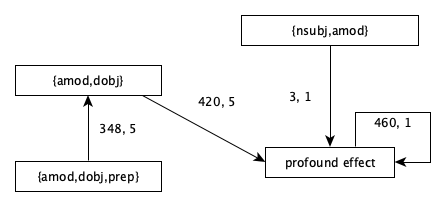
\includegraphics[width=\textwidth]{figures/pezik-img002.png}
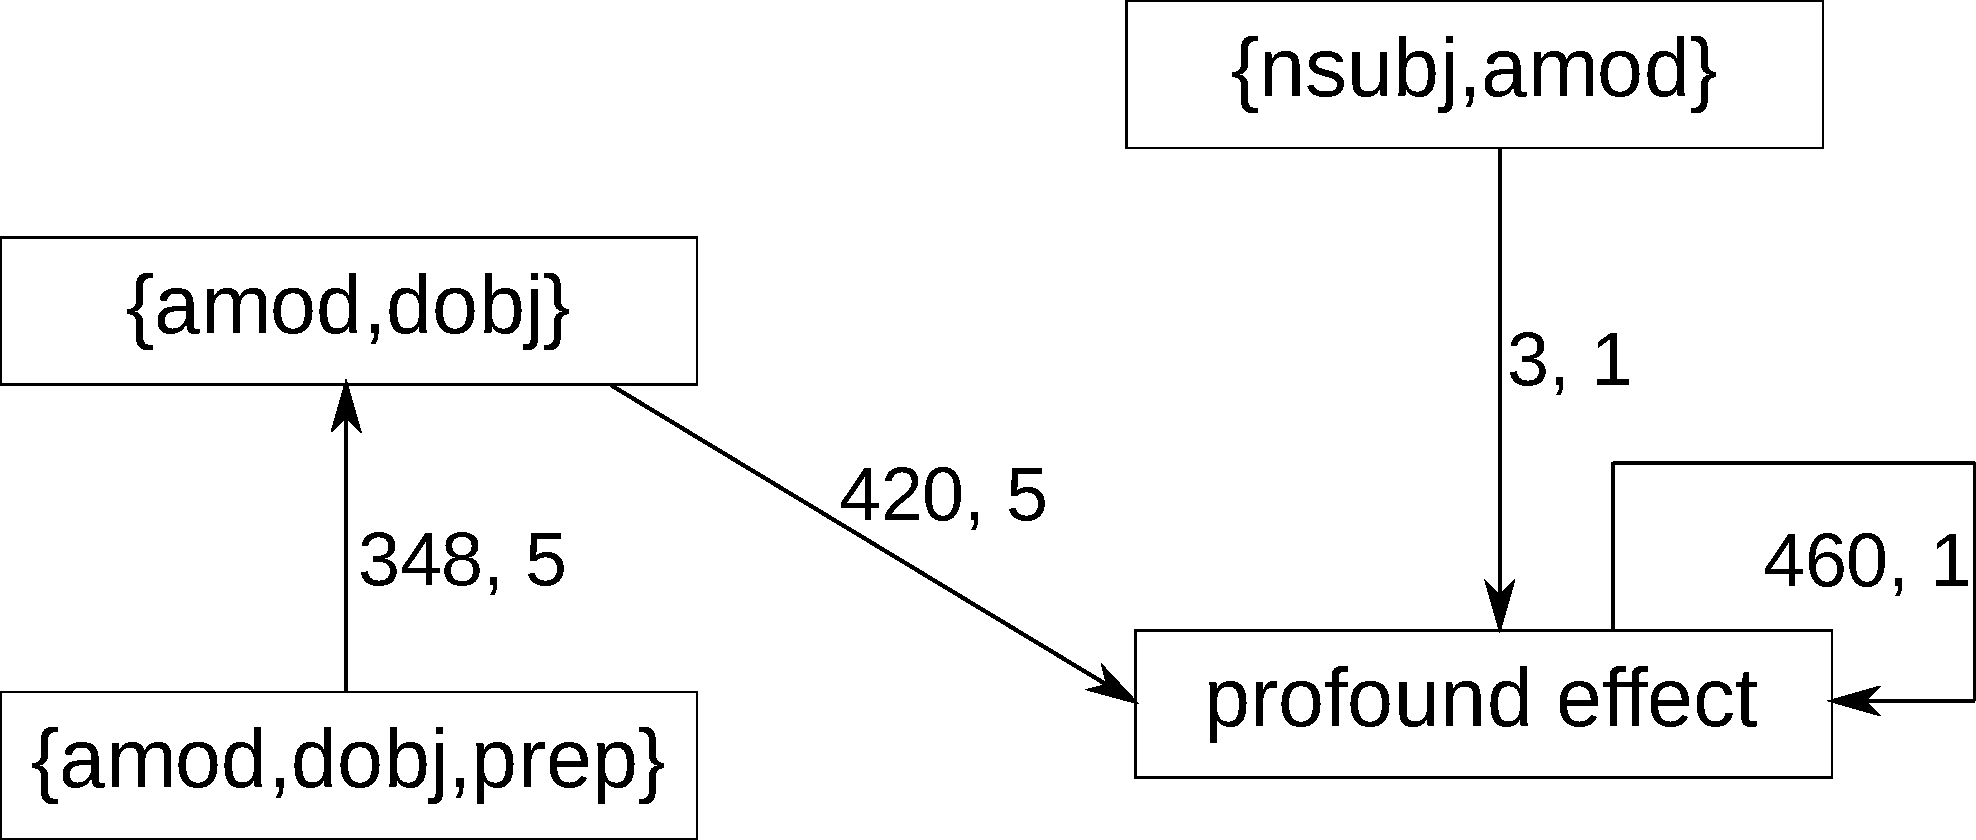
\includegraphics[width=.6\textwidth]{figures/pezik2.pdf}
\caption{Corpus-attested valency patterns on the subsumed collocation \textit{profound effect}\label{fig:pezik:2}}
\end{figure}

\largerpage[]
Complex restrictions on the potential valency of a given lexicalized subtree can be visualized as a syntactic subsumption graph similar to the one shown in \figref{fig:pezik:2}. As shown earlier in Tables~\ref{tab:pezik:3} and~\ref{tab:pezik:4}, the subsumed intensifying adjectival modifier collocation \textit{profound effect} is largely restricted to occur as a direct object (420/460 occurrences) of just 5 recurrent verbs, and when this is the case, it is in turn largely restricted to take a prepositional object (348/420). Such recurrent subsumption is conveniently represented as a subsumption graph.\footnote{The edge label \textit{420, 5} means that \textit{profound effect} occurs 420 times as a direct object of only 5 different verbs; The label \textit{3, 1} means that it is used only three times as a nominal subject with just one verb (\textit{to be}), etc.}






The examples discussed in this section show that both lexical and syntactic subsumption graphs provide an intuitive representation of such complex phenomena. As shown in the following sections, subsumption graphs can also be used to define the microstructure of entries in an automatic combinatorial dictionary.  

\section{Treelets}
The last section of this chapter presents the first version of \textit{Treelets} -- a new application which implements the dependency-based phraseology extraction and visualization methods described above. The application is distributed freely as a Docker image and can be used to extract one or more ACDs from a dependency-parsed reference corpus using user-defined dependency subtree patterns. The resulting ACDs can be searched through the built-in web application, exported or used directly as relational databases.

\subsection{Corpus formats and metadata}

The input formats currently supported by Treelets are: (1) plain text files with one text per line and (2) JSON Lines\footnote{See \url{http://jsonlines.org}.} format where each line contains a serialized dictionary with text metadata and contents. The metadata types supported include strings, floats, integers, text, dates and arrays of basic types, and they can be explicitly imported into the corpus database using the second format. It is therefore possible to preserve the original structure of the imported corpus at the level of bibliographic annotation and use it to create filtering or aggregating queries against the corpus database (see \tabref{tab:pezik:11}). It is also possible to provide externally parsed texts in the CoNLL-U format. Plain text files can be dependency-parsed with one of the spaCy\footnote{See \url{https://spacy.io}.} or UDPipe models (\citealt{StrakaStraková2017}). The largest corpus indexed so far with Treelets contains 500 million words, but the database backend of the application is fairly scalable and it is possible to index larger corpora.

\subsection{Defining extraction patterns}\label{sec:pezik:3.2}
Once a dependency-parsed corpus database is created and indexed, it is possible to define a set of syntactic patterns to be used in the process of extracting a combinatorial database. \tabref{tab:pezik:8} shows the result of using different extraction rules predefined in Treelets. The last two columns of the table show the number of extracted treelets and their cumulative frequencies. 


\begin{table}
\begin{tabularx}{\textwidth}{lQlrr}
\lsptoprule
\# & {Pattern}  & {Dependencies}  & {Treelets}  & {Occurrences}\\
\midrule
1 & Adjectival modifiers & amod & 405,385 & 4,090,711\\
2 & Nouns with prep. objects & prep, pobj & 368,357 & 1,906,280\\
3 & Direct objects & dobj & 275,037 & 2,562,868\\
4 & Nominal subjects & nsubj & 188,652 & 1,849,137\\
5 & Adjectival modifiers as direct objects & amod, dobj & 82,311 & 314,510\\
6 & Nominal subjects with adj. modifiers & nsubj, amod & 46,798 & 189,852\\
7 & Adverbial mods. of adjectives & advmod & 43,233 & 58,0021\\
8 & Adjectival mods. as direct objects with prep. & amod, dobj, prep & 20,082 & 70,545\\
9 & Direct Objects with Prep. Objects & amod, dobj, prep, pobj & 5,314 & 12,935\\
\lspbottomrule
\end{tabularx}
\caption{\label{tab:pezik:8} A summary of 8 syntactic types of subtrees extracted from BNC}
\end{table}

Custom extraction rules can be defined using the editor shown in \figref{fig:pezik:3}. In order to create a new extraction rule, which is essentially a dependency property subtree, it is necessary to define a directed tree graph as well as the aggregation keys of its vertices and edges. By default, the aggregation key is a combination of lemmas, part of speech tags and dependency types defined on the edges of the graph.

  
\begin{figure}
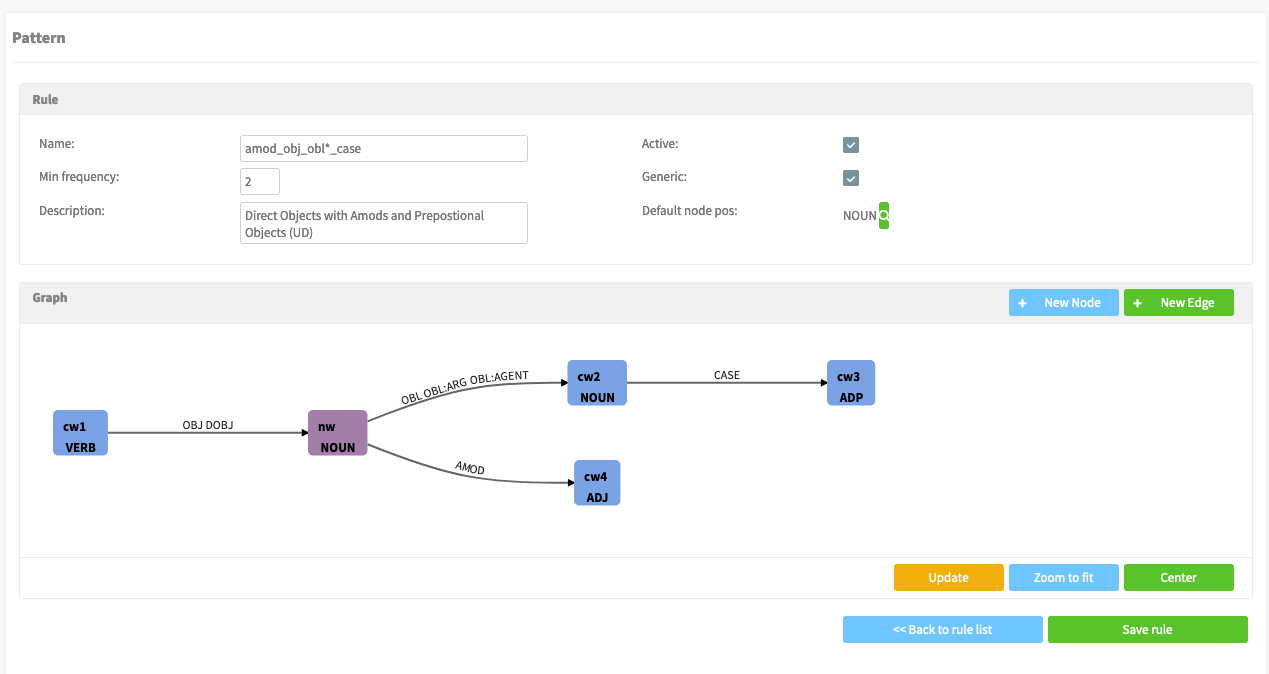
\includegraphics[width=\textwidth]{figures/pezik-img003.png}
\caption{Designing extraction patterns in Treelets.\label{fig:pezik:3}}
\end{figure}

The rule shown in \figref{fig:pezik:3} illustrates a special feature of Treelets which was implemented to deal with possible peculiarities of different dependency treebank annotation schemes. As hinted above, the validity of the continuity restraint, which assumes that phraseological units are lexicalized subtrees of the sentence dependency tree, may depend on the details of the dependency formalism. For example, in the current version of the Universal Dependency framework prepositions may function as case markers of their nominal heads. This means that the continuity restraint is not preserved for constructions such as \textit{have a direct bearing on}. This is because the governor nominal node whose case is marked by the preposition \textit{on} according to this representation is not an ``obligatory'' or ``typical'' lexical node of this expression.\footnote{This example also shows that the results of relational phraseology extraction depend on the syntactic framework used to annotate a given corpus.} To deal with such discontinuities, it is possible to use part-of-speech tags rather than lemmas to define the aggregation keys on whose values the extraction pattern is aggregated. In the example extraction pattern shown in \figref{fig:pezik:3}, the aggregation key of the vertex marked as \textit{cw2} is therefore simply its part-of-speech tag (NOUN) rather than a combination of the tag and a lemma found on this vertex. In other words, the lemmas on the \textit{cw2} vertex are ignored in the aggregation process and constructions such as \textit{have a direct bearing on} + NOUN are counted as instances of the same lexicalized pattern. It is possible to test such rules on a selected reference corpus before using them for extraction. Once the ACD is generated, it can be searched for both headwords such as \textit{role} as a noun and specific treelets of arbitrary length in which it is found such as \textit{play a specific role in the development of}. One of the results of a single query term for the string \textit{role} in the ACD search field is a view similar to \tabref{tab:pezik:9}, which summarizes the syntactic types of the lexicalized treelets of the noun \textit{role} in the ACD extracted from BNC.\footnote{\textrm{Currently, syntactic variants of recurrent treelets such as} \textrm{\textit{high hopes}} \textrm{vs} \textrm{\textit{hopes were/are high}} \textrm{are not explicitly related in the underlying database. However, they are usually dynamically related in user queries. For example a search for the lemma \textit{hope} will return both of the above-mentioned syntactic configurations of \textit{high} + \textit{hopes} in the summary table of results similar to \tabref{tab:pezik:9}.}} 

\begin{table}
\begin{tabularx}{\textwidth}{lQrQ}
\lsptoprule
{\#}  & {Rule}  & {Treelets}  & {Examples}\\\midrule
 1 & Nouns with prep. objects &  1,182 & \textit{role of state, role in society, role in process}\\
 2 & Adjectival modifiers &  504 & \textit{important role, major role, key role}\\
 3 & Adjectival mods. as direct objects &  367 & \textit{play important role, play major role, play key role}\\
 4 & Direct objects &  334 & \textit{meet role, play role, have role}\\
 5 & Adjectival mods. as direct objects with preps. &  168 & \textit{play important role in, play major role in, play key role in}\\
 6 & Nominal subjects &  106 & \textit{role be, role have}\\
 7 & Direct objects with prep. objects &  91 & \textit{play important role in development, play central role in development}\\
 8 & Nominal subjects with adjectival mods. &  53 & \textit{initial role be, former role be, final role be}\\
\lspbottomrule
\end{tabularx}
\caption{\label{tab:pezik:9}A summary of recurrent subtrees containing the noun \textit{role}}
\end{table}

By clicking on a matching treelet, users are redirected to its dedicated page which currently consists of the following four sections:

\begin{itemize}
\item The concordances of the recurrent treelet in the reference corpus;
\item The statistics table with some statistical properties of the treelet, such as frequency, dispersion and strength of association;
\item The dependency structure of the candidate construction;
\item The valency section, which features a tabular view of the directly subsumed and directly subsuming recurrent treelets. For example, the binary collocation \textit{important role} is hyperlinked to the entry page for \textit{play an important role}, which is linked to the entry for \textit{play an important role in}, etc.
\end{itemize}

The Valency section showcases a simple application of the subsumption graph structure of the ACD entries generated with Treelets. More sophisticated representations of the higher-order constructions detected with this application are discussed in the next section.

The current version of Treelets also supports extraction bases on untyped dependency tree patterns. In this mode, users only define lemmas for which all dependency subtrees up to a certain size (the current limit being six nodes) are extracted, aggregated and ordered by their frequency. In other words, only the \textbf{shape} of extracted subtrees, i.e. directed edges between the nodes, is predefined in this case. \tabref{tab:pezik:10} shows the results of such ad-hoc extraction of recurrent subtrees containing the noun \textit{factor} in the BNC. Combinations of nouns joined by a preposition turn out to be the most productive pattern in which \textit{factor} is found in this corpus with 254 distinct recurrent treelets identified. The largest number of instances is yielded by combinations of adjectives modifying this noun with 7,962 occurrences identified.

\begin{table}[t]
\begin{tabularx}{\textwidth}{llrrQ}
\lsptoprule
\# & Structure & Subtrees & Mass & Examples\\\midrule
1  & v2-prep-v1-pobj->v0 & 254 & 3,104 & number + of + factor\linebreak one + of + factor\linebreak depend + on + factor\\
2  & v0-amod->v1 & 218 & 7,962 & key + factor\linebreak important + factor\linebreak major + factor\\
3  & v1-dobj->v0 & 153 & 1,087 & take + factor\linebreak identify + factor\linebreak consider + factor\\
4  & v1-nsubj->v0 & 120 & 2,730 & factor + be\linebreak factor + include\linebreak factor + influence\\
5  & v2-pobj-v0-amod->v1 & 74 & 1,292 & of + other + factor\linebreak by + other + factor\linebreak of + important + factor\\
\lspbottomrule
\end{tabularx}
\caption{\label{tab:pezik:10}Weakly-supervised extraction of dependency subtrees}
\end{table}

\subsection{Exploring valency patterns}

To illustrate the exploratory potential of subsumption graph visualizations, let us consider graphs generated for two entries from two different corpora. \figref{fig:pezik:4} shows a subsumption graph generated for the noun \textit{role} from BNC using the eight extraction rules mentioned above. Only subtrees which occurred in this corpus at least twice are shown in this graph. The two vertices with the highest indegree in this graph represent the direct object binary collocations \textit{play a role} and \textit{have a role}. 

  
\begin{figure}[t]
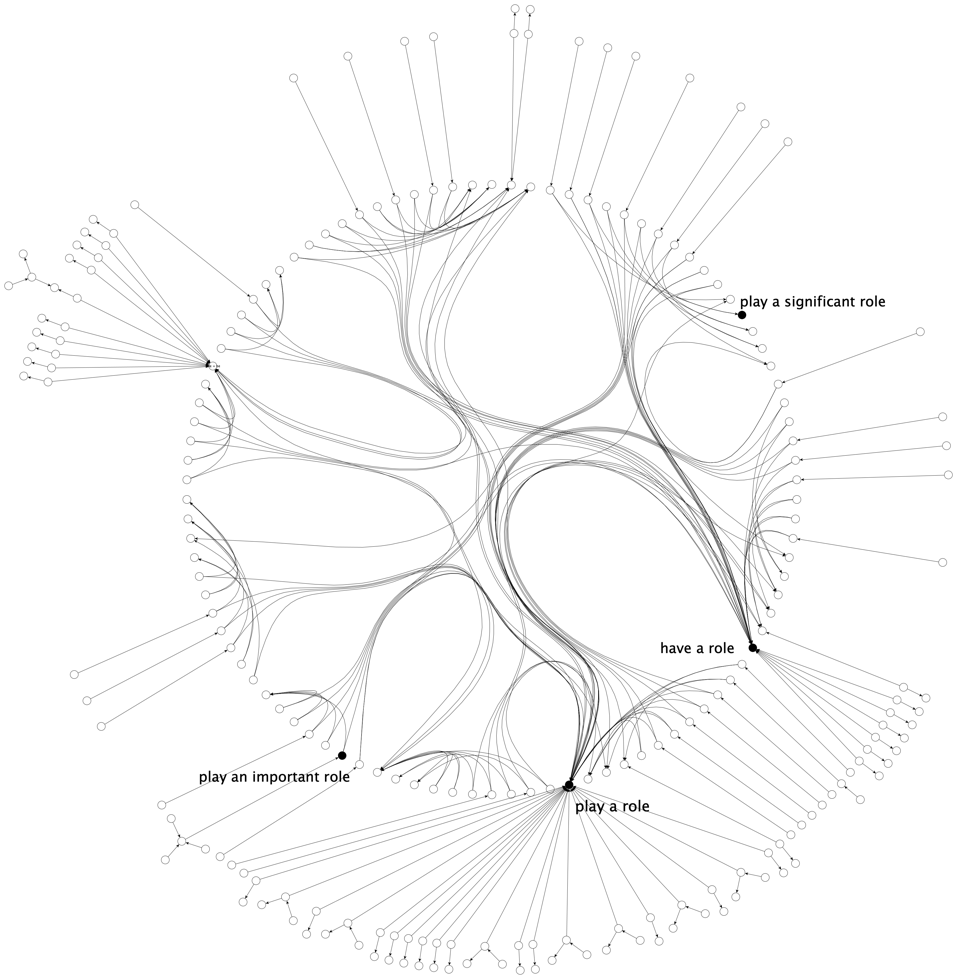
\includegraphics[width=\textwidth]{figures/pezik-img004.png}
\caption{A subsumption graph of \textit{role} as a noun generated from the BNC. Only selected treelets are labelled.\label{fig:pezik:4}}
\end{figure}


\begin{table}
\begin{tabular}{lrr rr}
\lsptoprule
& \multicolumn{2}{c}{Indegree} & \multicolumn{2}{c}{Frequency}\\\cmidrule(lr){2-3}\cmidrule(lr){4-5}
ACD & BNC & COCA & BNC & COCA\\\midrule
play a role & 99 & 292 & 2,591 & 16,225\\
have a role & 96 & 136 & 1,042 & 2,955\\
\lspbottomrule
\end{tabular}
\caption{\label{tab:pezik:11}Frequency and \textit{productivity} of play/have a role in COCA and BNC}
\end{table}

As shown in \tabref{tab:pezik:11}, \textit{play a role} is considerably more frequent than \textit{have a role} in COCA and only slightly more frequent in the BNC. The indegrees of those vertices in the subsumption graph suggest that \textit{play a role} is used in various larger constructions in COCA and BNC. The exact structure of the subsumption graph depends on the size and composition of the corpus, especially if a raw frequency threshold is used to select the nodes. In principle, it is also possible to use any conjunction of frequency, strength of association, dispersion and independence scores to create more sophisticated criteria of selecting the vertices of a subsumption graph. For example, a subsumption graph could contain only vertices representing subtrees whose average strength of association score is greater than some minimum \textbf{significance} threshold. Even a simple frequency-based subsumption graph may be helpful in formulating hypotheses to explain the differences between the varieties of English represented by the three corpora. One such hypothesis could be that \textit{play a role} is more frequent in American English than in British English or simply in the registers and text types represented in the two reference corpora.

\subsection{Source databases}

The corpora and ACDs generated by Treelets are stored in a PostgreSQL database, which can be installed on any machine and in any location specified by the user. This means that more technical users can take full advantage of the dependency-parsed corpus database by querying it directly and from different client applications if necessary to obtain data views which have not yet been implemented in the Treelets web application. One example of such a query against the source corpus database is shown in \figref{fig:pezik:12}. The purpose of the query is to find dependency subtrees which consist of the preposition \textit{of}, the noun \textit{force} as its object and an unspecified adjectival modifier or compound noun dependent of this object. Furthermore, the search is limited to texts which are marked as ``SPOK'' (spoken register in the imported COCA corpus). The results are aggregated on lemmas and dependency types, counted and limited to matching prepositional phrases which only occur in at least 20 different spoken texts in the corpus.

\begin{figure}[p]
\begin{lstlisting}[language=SQL,frame=lines]
SELECT
wc1.head_lemma gov_lemma,  wc2.lemma dep_lemma,  wc1.lemma lemma, 
wc1.dep dep, wc2.dep dep_dep, count(*) cnt, count(distinct(wc1.text_id)) texts

FROM
word_conllu wc1
JOIN word_conllu wc2 on wc2.sentence_id = wc1.sentence_id and wc2.head_id = wc1.id
JOIN text t on t.id = wc1.text_id

WHERE
wc1.lemma = 'force' AND wc1.head_lemma='of'
AND wc2.dep = ANY(ARRAY['amod','compound']) AND wc1.dep = ANY(ARRAY['pobj'])
AND t.genre = ANY(ARRAY['SPOK'])
GROUP BY wc1.lemma,wc1.head_lemma, wc1.dep,dep_dep,dep_lemma
having count(distinct(wc1.text_id)) >= 50
order by cnt desc;
\end{lstlisting}
\caption{\label{fig:pezik:12}An SQL query used to extract and aggregate recurrent prepositional attachments from the Treelets corpus database.}
\end{figure}


\begin{table}[p]
\begin{tabular}{lllllrr}
\lsptoprule
\texttt{gov\_lemma} & \texttt{dep\_lemma} & \texttt{lemma} & \texttt{dep} & \texttt{dep\_dep} & \texttt{cnt} & \texttt{texts}\\
\midrule
of & armed & force & pobj & amod &  197 &  167\\
of & military & force & pobj & amod &  174 &  155\\
of & work & force & pobj & compound &  134 &  122\\
of & task & force & pobj & compound &  133 &  112\\
of & U.S. & force & pobj & compound &  124 &  112\\
\lspbottomrule
\end{tabular}
\caption{\label{tab:pezik:13}Recurrent prepositional attachments retrieved from the Treelets corpus database}
\end{table}


As shown in \tabref{tab:pezik:13}, the most frequent prepositional attachments identified with this query include \textit{of armed forces}, \textit{of military forces}, \textit{of (det) work force}, etc. The query could be easily elaborated to identify more complex subtrees or return concordances of matching spans instead of aggregated summaries. It is also possible to relax the dependency joins defined in the query and use positional cooccurrence criteria in order to increase the recall of queries by matching unspecified or erroneously parsed dependency relations.


\section{Summary and future work}

The starting assumption of this paper was the vast majority of phraseological units have an internal syntactic structure and that subsentential PUs have an external valency. Using a dependency-based phraseology extraction approach, the paper then demonstrated how those properties of PUs can be at least partly accounted for in automatically combinatorial databases. It is hoped that the software tool implementing dependency-based phraseology extraction may help lexicographers and phraseologists “deal with the enormous structural variety of English idioms” \citep[11]{CowieEtAl1993} and possibly also explore prefabricated collocational chains as a noteworthy type of phraseological units. Future versions of Treelets will also include phraseology detection features \citep{Pęzik2018} to enable more advanced reference corpus-based indexing of idiomatic expressions.

{\sloppy\printbibliography[heading=subbibliography,notkeyword=this]}
\end{document}
